\documentclass[11pt]{report}

% Basic Packages
\usepackage[a4paper, margin=2.5cm]{geometry}
\usepackage[utf8]{inputenc}
\usepackage{graphicx}
\usepackage{amsmath}
\usepackage{indentfirst}
%\usepackage[backend=biber, style=numeric, sorting=none]{biblatex} % APA with numeric citations
%\addbibresource{References.bib} % Import the bibliography file
\usepackage[numbers]{natbib} % Use numeric citations
\bibliographystyle{unsrt} % Specify bibliography style
\usepackage{caption}
\usepackage{tocloft}
\usepackage{adjustbox}
\usepackage{float}
\usepackage{longtable}
\usepackage{blindtext}
\usepackage{titlesec}
\usepackage{textcomp}
\usepackage[table]{xcolor} % For shading cells
\usepackage{array}         % For custom column widths
\usepackage{multirow, colortbl}
\usepackage{booktabs}
\usepackage{rotating}
\usepackage{graphicx}
\usepackage{pifont}  % For \checkmark and \xmark
\usepackage{amssymb} 
\usepackage{fancyhdr} % For custom page numbering
\usepackage{placeins} % This forces LaTeX to place all preceding floats before continuing with regular text.
\usepackage{titlesec} % optional, for more control over formatting
\usepackage{etoolbox} % for patching macros safely
\usepackage{xurl}  % Allows line breaks in URLs at more places

\newcommand{\degree}{\ensuremath{^\circ}}

% Adjust caption spacing
\setlength{\abovecaptionskip}{3pt}
\setlength{\belowcaptionskip}{5pt}
\captionsetup{font=scriptsize, justification=centering}

% Hyperref for links
\usepackage[colorlinks=true, linkcolor=black, urlcolor=blue, citecolor=black]{hyperref}

% Optional Table Support
\usepackage{array, tabularx, xcolor, booktabs}

% Line Spacing
\usepackage{setspace}
\renewcommand{\baselinestretch}{1.5}

% Font Setup
\usepackage{mathptmx}

% Rename "Contents" to "Table of Contents"
\renewcommand{\contentsname}{Table of Contents}

% Redefine section numbering
\renewcommand{\thesection}{\arabic{section}}
\renewcommand{\thesubsection}{\thesection.\arabic{subsection}}
\renewcommand{\thesubsubsection}{\thesubsection.\arabic{subsubsection}}
\setcounter{secnumdepth}{3}
\setcounter{tocdepth}{3}

% Customize the ToC title
\renewcommand{\cfttoctitlefont}{\normalfont\Large\bfseries}
\setlength{\cftbeforetoctitleskip}{-1em}
\setlength{\cftaftertoctitleskip}{1em}

% Redefine Bibliography Title to Use Section-Level Formatting
\makeatletter
\renewcommand{\chapter}{\@startsection{section}{1}{\z@}{-3.5ex \@plus -1ex \@minus -.2ex}%
  {2.3ex \@plus.2ex}{\normalfont\Large\bfseries}}
\makeatother

% Adjust Figure/Table numbering format in ToC
\renewcommand{\cftfigpresnum}{Figure~}
\renewcommand{\cfttabpresnum}{Table~}
\renewcommand{\cftfigaftersnum}{ - }
\renewcommand{\cfttabaftersnum}{ - }

\setlength{\cftfignumwidth}{3cm} % Adjust width for figure numbers
\setlength{\cfttabnumwidth}{3cm} % Adjust width for table numbers

% Redefine List of Figures/Table Titles as Section-Style
\usepackage{etoolbox} % For removing list headers from ToC

% Make List of Figures and List of Tables titles match "section" format
\titleformat{\listfigurename}[block]{\Large\bfseries}{}{0pt}{}
\titleformat{\listtablename}[block]{\Large\bfseries}{}{0pt}{}

% Prevent List of Figures/Tables from appearing in the ToC
\patchcmd{\listoffigures}{\chapter*}{\section*}{}{}
\patchcmd{\listoftables}{\chapter*}{\section*}{}{}

% Define custom page styles for List of Figures and Tables
\fancypagestyle{figures}{
    \fancyhf{}
    \fancyfoot[C]{F-\thepage} % Custom page numbering for figures
    \renewcommand{\headrulewidth}{0pt}
    \renewcommand{\footrulewidth}{0pt}
}

\fancypagestyle{tables}{
    \fancyhf{}
    \fancyfoot[C]{\thepage} % Default page numbering for tables
    \renewcommand{\headrulewidth}{0pt}
    \renewcommand{\footrulewidth}{0pt}
}



\begin{document}
    \begin{titlepage}
        \centering
        % University Logo
        
\includegraphics[width=0.3\textwidth]{Figures/Logo_UA.png}\\[1cm] 
    
        % University Name
        {\Large \textbf{Universidade de Aveiro (University of Aveiro)}}\\[1cm]
    
    
        % Document Title
        {\Large \textbf{Supplementary Technical Repository}}\\[1cm]
    
        % Subject
        {\large Projeto em Engenharia Aeroespacial (Project in Aerospace Engineering) - 42260}\\[.5cm]

        % Departments
        {\small
            \textbf{DETI} - Departamento de Eletrónica, Telecomunicações e Informática \\
            (Department of Electronics, Telecommunications, and Informatics)\\
            \textbf{ESAN} - Escola Superior Aveiro Norte \\
            (Aveiro North School)
        }\\[1cm]
    
        % Student Names and Numbers
        \begin{flushleft}
            \textbf{Students:}\\
            - Diogo Gavancho (113078)\\
            - Diogo Ribeiro (108217)\\
            - Márcio Teixeira (114074)\\
            - Rui Alho (113992)\\[1cm]
        
            \textbf{Advising Professors:}\\
            - Prof. Paulo Lima\\
            - Prof. Ricardo Torcato\\[1cm]
        
            \textbf{Subject Coordinator:}\\
            - Prof. Pedro Casau\\[2cm]
        \end{flushleft}
    
        % Date
        \vfill
        {\large Date: June 2025}
    
        \thispagestyle{empty}
    \end{titlepage}

    % Table of Contents (start numbering)
    \pagenumbering{roman} % Optional: Use Roman numerals for TOC
    \tableofcontents
    \clearpage

    \pagenumbering{arabic} % Restart numbering with Arabic numerals
    \setcounter{page}{1} % Start numbering from 1

    \section{Introduction To Repository}
This document contains supplementary information related to the report Development of a Mechanical Structure for a Planetary Exploration Rover Based on Direct Digital Manufacturing. Although the content presented here is not essential for understanding the main body of the report, it provides relevant technical details and extended material that support and contextualize the project. The information is organized according to the structure of the main report, with each part corresponding to the respective section, as indicated.

    \renewcommand{\thesection}{S3}
\section{Design Basis: State of the Art, Requirements \& Specifications, and Benchmarking}

\subsection{State-of-the-Art Rovers in Planetary Exploration}

    \subsubsection{Zhurong: Active Suspension for Adaptability}
        Figure \ref{fig:Zhurong} shows China's Zhurong rover, which features an advanced active suspension system that independently adjusts each wheel's position and load \cite{CNSA_Zhurong}. This design improves performance on loose soils and steep inclines, such as those found in Mars' Utopia Planitia region.
        
        Its aluminum-silicon carbide composite wheels are lightweight yet strong, while its six-wheeled configuration reduces ground pressure \cite{Zhurong_Mission_Analysis_2021}. On Titan, where gravity is lower than Earth's, and the surface includes methane lakes and frozen ground, an active suspension system could enhance the ability to navigate these diverse terrains. Zhurong's approach highlights the importance of independent control for achieving stability and mobility.

        \renewcommand{\thefigure}{S1}
        \begin{figure}[ht]
            \centering
            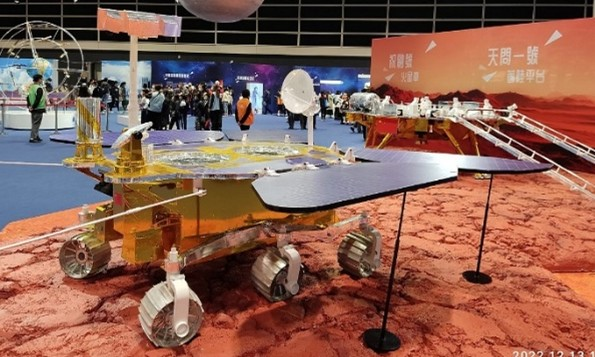
\includegraphics[height=6cm]{Figures/Zhurong.jpg}
            \caption{Full-scale mockup of Zhurong rover \cite{Wikipedia_Zhurong}. Image by AKAMGO yalms (CC BY-SA 4.0).}
            \label{fig:Zhurong} 
        \end{figure}
        \vspace{-20pt} % Adjust this value to reduce the space
        \FloatBarrier

    \subsubsection{VIPER: Navigating the Lunar South Pole}
        NASA's VIPER rover, presented in Figure \ref{fig:VIPER}, is tailored to operate in the extreme environment of the Moon's south pole \cite{NASA_Viper_Project}. It uses a four-wheel independent suspension system with active articulation, enabling precise manoeuvring such as "crab-walking" over steep slopes and loose regolith.
        
        VIPER's design incorporates lightweight composites and advanced thermal systems to withstand temperature extremes and abrasive lunar dust \cite{NASA_Viper_Rover}. With its cryogenic temperatures and potential for surface liquid hydrocarbons, Titan's environment would benefit from similar thermal management solutions. VIPER's mobility system also suggests how active articulation could address Titan's challenging topography.

        \renewcommand{\thefigure}{S2}
        \begin{figure}[ht]
            \centering
            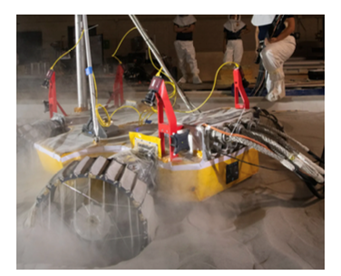
\includegraphics[height=6cm]{Figures/VIPER.png}
            \caption{The VIPER engineering team observe the rover prototype’s ability to navigate the fluffy lunar soil simulant in the SLOPE lab at NASA’s Glenn Research Center in Cleveland \cite{NASA_Viper_Prototype}.}
            \label{fig:VIPER} 
        \end{figure}
        \vspace{-20pt} % Adjust this value to reduce the space
        \FloatBarrier

    \renewcommand{\thesection}{S4}
\section{Conceptual Design}

\subsection{Mobility System Subdivision}

    \subsubsection{Traction Subsystem}
        The traction subsystem generates the forces to move the vehicle across the terrain. During the research phase, several solutions for this subsystem were identified, including wheels (the most common solution), tracks, legs, hybrid drives, and screw propulsion.
        
        Traditional wheels typically employ pneumatic tires, which are synthetic or natural rubber and consist of a tread for traction and a body that contains compressed air \cite{Wikipedia_Tire}. However, for space exploration missions, other types of tires are more relevant to the mission context. These include tires made of a metallic mesh with treads attached that do not require pressurized gas. Such tires are constructed from shape-memory alloys, with nickel-titanium alloys being the most common due to their durability and ability to retain shape.

        In addition, rigid wheels without tires are frequently used in space exploration missions. For example, NASA's Perseverance and Curiosity rovers employ rigid wheels to navigate challenging terrain effectively. The most common wheel configuration for rovers is six wheels, which allows for redundancy in case of wheel failure. However, newer exploration vehicles like Venturi's FLEX rover have adopted a four-wheel configuration.

        Figure \ref{fig:Wheels} presents three types of wheels used in space exploration. The wheel on the left features a metallic net structure made of nickel-titanium alloy (Nitinol), which is used on the FLEX rover. The two wheels on the right are rigid wheels with solid surfaces employed on NASA's Curiosity and Perseverance rovers.

        \renewcommand{\thefigure}{S3}
        \begin{figure}[ht]
            \centering
            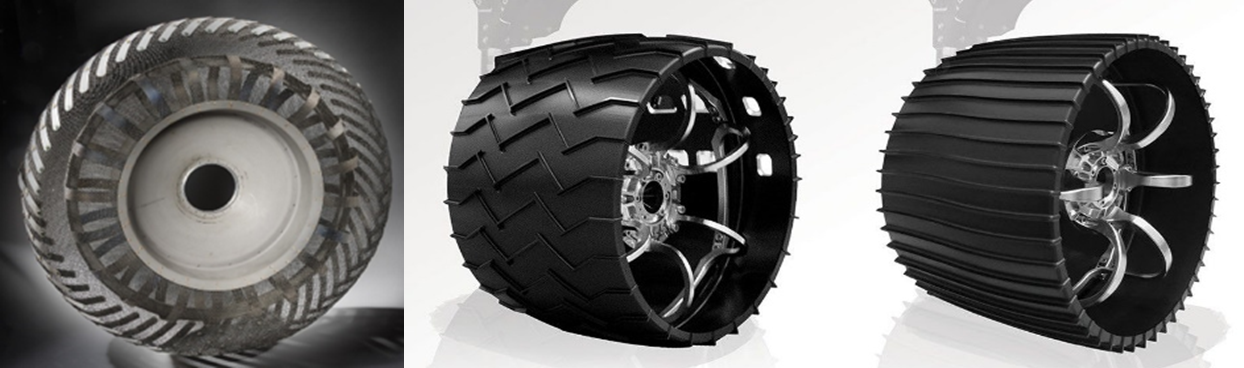
\includegraphics[height=3cm]{Figures/Wheels.png}
            \caption{Three different types of wheels used in space exploration missions. The wheel on the left possesses a net structure made of a nitinol alloy and was used on the FLEX rover \cite{Smithsonian_Lunar_Rover}. The next two wheels have a rigid soil contact surface and were used on NASA’s Curiosity and Perseverance rovers respectively \cite{NASA_Wheels}.}
            \label{fig:Wheels} 
        \end{figure}
        \vspace{-20pt} % Adjust this value to reduce the space
        \FloatBarrier

        Tracks utilize a continuous band of track plates or treads driven by wheels, allowing for more significant surface contact. More modern iterations of this technology can utilize soft belts of synthetic rubber, but the more classical type of track is a chain track made of steel plates \cite{PopularScience_TankTread_1944}. Figure \ref{fig:Tracks} shows an example of an exploration vehicle operating with tracks.

        \renewcommand{\thefigure}{S4}
        \begin{figure}[ht]
            \centering
            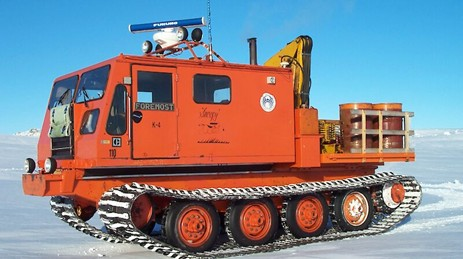
\includegraphics[height=4cm]{Figures/Track.jpg}
            \caption{Tracked exploration vehicle used to support scientific and other field programs \cite{Australian_Antarctic_TrackedVehicles}.}
            \label{fig:Tracks} 
        \end{figure}
        \vspace{-20pt} % Adjust this value to reduce the space
        \FloatBarrier

        Legs mimic animal-like walking or crawling using actuators as articulations. These types of systems are rather complex and are still an object of study, as most are still experimental prototypes or proofs of concept \cite{Wikipedia_WalkingVehicle}. A perfect example is the legged walker used by the U.S. Army, represented in Figure \ref{fig:Tracks}.

        \renewcommand{\thefigure}{S5}
        \begin{figure}[ht]
            \centering
            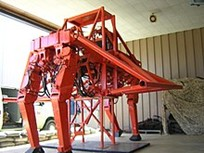
\includegraphics[height=4cm]{Figures/Legs.jpg}
            \caption{Legged quadruped walker on display at the U.S. Army Transportation Museum \cite{Wikipedia_WalkingVehicle}.}
            \label{fig:Legs} 
        \end{figure}
        \vspace{-20pt} % Adjust this value to reduce the space
        \FloatBarrier

        Hybrid drive combines both wheels or tracks with legs and there is little to no research made on this type of system being a technology that is even less developed than legs. Figure \ref{fig:Hybrid} presents Hyundai's hybrid drive car concept, "Elevate", which combines wheels with legs to enhance mobility across challenging and uneven terrains \cite{Hyundai_Technology}.

        \renewcommand{\thefigure}{S6}
        \begin{figure}[ht]
            \centering
            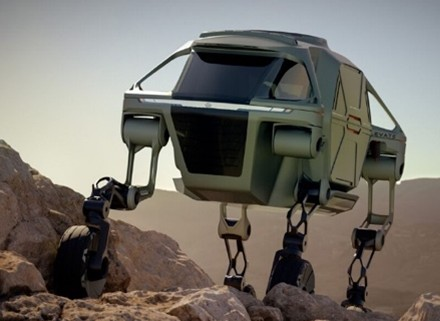
\includegraphics[height=4cm]{Figures/Hybrid.jpg}
            \caption{Hyundai’s hybrid drive car concept “Elevate” \cite{Hyundai_Technology}.}
            \label{fig:Hybrid} 
        \end{figure}
        \vspace{-20pt} % Adjust this value to reduce the space
        \FloatBarrier

        Screw-propelled vehicles utilize long, continuously rotating screws to move. This type of system allows for an amphibious vehicle that can also cope with challenging terrain \cite{Wikipedia_ScrewPropelledVehicle}. Figure \ref{fig:Screw} shows the ZIL-2906, a Russian-made amphibious vehicle that employs a screw drive system to navigate challenging terrains and amphibious environments \cite{Wikipedia_ZIL2906}.

        \renewcommand{\thefigure}{S7}
        \begin{figure}[ht]
            \centering
            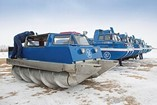
\includegraphics[height=4cm]{Figures/Screw.jpg}
            \caption{“ZIL-2906” a Russian made amphibious vehicle that utilizes the screw drive system \cite{Wikipedia_ZIL2906}.}
            \label{fig:Screw} 
        \end{figure}
        \vspace{-20pt} % Adjust this value to reduce the space
        \FloatBarrier
        
    \subsubsection{Steering Subsystem}
        The steering on these vehicles is almost exclusively done by independent motors that individually turn each point of contact with the ground. Most commonly on these missions, the points of contact are six wheels, the parameter that varies between them is the number of contacts that effectively turn. That number could range from all the points of contact (All-steer), to only the points of contact on the front and the back (Dual-steer), to the ones on the front of the craft (Front-steer), to even no steering on the points of contact (No-steer).
        
	    The No-steer systems turn by rotating all the elements on one side one way and the ones on the other side the opposite way. This creates a torque on the vertical axis that goes through the geometric centre of all points of contact and turns the vehicle. This mechanism is mostly used by tracked vehicles like tanks.


    \subsubsection{Spring Subsystem}
        The spring subsystem consists of, as the name implies, springs that act as the primary elastic component to absorb and store energy from road impacts. Besides significantly reducing the vibrations transferred to the vehicle, they also improve tire contact with the surface. There are several types of springs that can be employed, those being: mechanical springs; air springs; and magnetic springs \cite{EngineersPost_SuspensionSprings}.
        
        Mechanical springs work through the elastic properties of the material they are made of, by displacing it, or deforming it, the material exerts a force so that it returns to its original shape. This category includes traditional coil springs, commonly used in standard vehicles, as shown in Figure \ref{fig:Spring}, and torsion bars, which provide similar elastic functionality. 

        \renewcommand{\thefigure}{S8}
        \begin{figure}[ht]
            \centering
            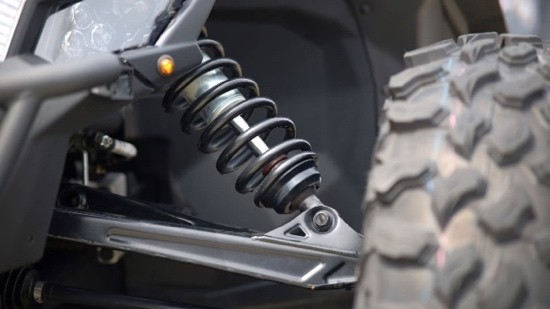
\includegraphics[height=4cm]{Figures/Spring.jpg}
            \caption{Classical type of vehicle suspension springs \cite{Tevema_SuspensionSprings}.}
            \label{fig:Spring} 
        \end{figure}
        \vspace{-20pt} % Adjust this value to reduce the space
        \FloatBarrier
        
    	Air springs, like the ones represented in Figure \ref{fig:AirSpring}, consist of compressed air in flexible bags. As these bags are compressed, the pressure inside rises and offers greater resistance to further deformation; the opposite is also true if the bags are expanded. These springs allow for both an adjustable ride height and an adjustable stiffness \cite{Vibracoustic_AirSprings}.

        \renewcommand{\thefigure}{S9}
        \begin{figure}[ht]
            \centering
            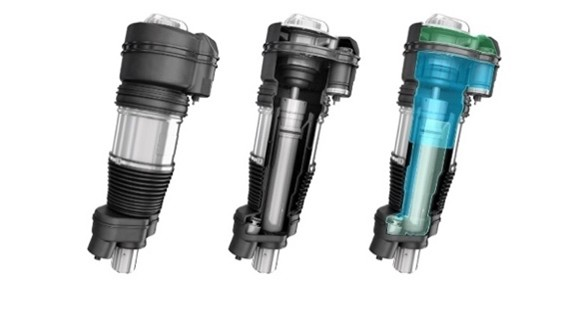
\includegraphics[height=4cm]{Figures/AirSpring.jpg}
            \caption{Vibracoustic’s switchable three-chamber air springs \cite{Vibracoustic_AirSprings}.}
            \label{fig:AirSpring} 
        \end{figure}
        \vspace{-20pt} % Adjust this value to reduce the space
        \FloatBarrier

        Magnetic springs utilize powerful magnets to generate magnetic fields that generate either repulsive or attractive forces. In theory, these springs also have the advantage of not needing any type of dampening system, as they act as their own shock absorbers. Figure \ref{fig:MagneticSpring} represents the schematic of a magnetic car suspension \cite{GreenCarCongress_ElectricTruck_2008}.

        \renewcommand{\thefigure}{S10}
        \begin{figure}[ht]
            \centering
            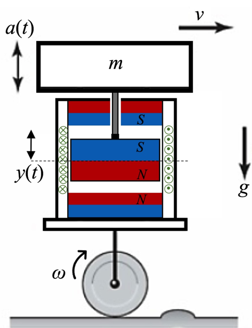
\includegraphics[height=4cm]{Figures/MagneticSpring.png}
            \caption{Model of a magnetic car suspension spring \cite{GreenCarCongress_ElectricTruck_2008}.}
            \label{fig:MagneticSpring} 
        \end{figure}
        \vspace{-20pt} % Adjust this value to reduce the space
        \FloatBarrier

    \subsubsection{Damper Subsystem}
        Shock absorbers, or dampers, are often integrated with springs to control the oscillations created by them and dissipate energy \cite{FastCar_Dampers}. They fulfil this purpose by converting kinetic energy into another form, most commonly thermal energy, and dissipating it as heat \cite{MotorsAndManStuff_Dampers}. There are several damper systems, including hydraulic, pneumatic, magnetorheological, friction disk, electromagnetic, hydropneumatic, and hysteresis.
        
	    Hydraulic dampers, like the one in Figure \ref{fig:HydraulicShockAbsorber}, are the most common in the automotive market. They compress a hydraulic fluid, which in turn heats it, converting the kinetic energy and then dissipating it through heat. This type of system may employ special internal valving that allows the adjustment of the strength of dampening based on compression or extension.

        \renewcommand{\thefigure}{S11}
        \begin{figure}[ht]
            \centering
            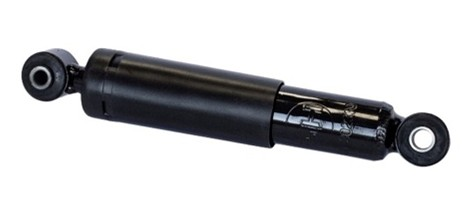
\includegraphics[height=3cm]{Figures/HydraulicShockAbsorber.jpg}
            \caption{Hydraulic shock absorber for leaf spring trailers \cite{Jia2018_MagneticSpring}.}
            \label{fig:HydraulicShockAbsorber} 
        \end{figure}
        \vspace{-20pt} % Adjust this value to reduce the space
        \FloatBarrier

        Pneumatic shock absorbers work on a similar principle to hydraulic ones, except instead of compressing a hydraulic fluid, they compress the gas, the most used being nitrogen. Because gas is compressible, the equipment involved is less susceptible to shock damage. Figure \ref{fig:PneumaticShockAbsorber} illustrates a perfect example of a pneumatic damper.

        \renewcommand{\thefigure}{S12}
        \begin{figure}[ht]
            \centering
            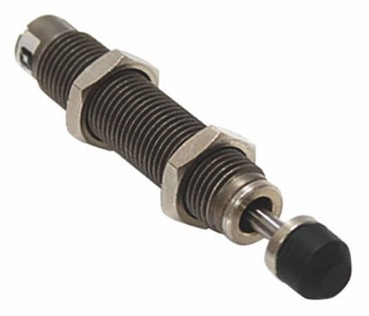
\includegraphics[height=3cm]{Figures/PneumaticShockAbsorber.jpg}
            \caption{RS PRO Shock Absorber, 67mm Body Length pneumatic damper \cite{RSComponents_ShockAbsorber}.}
            \label{fig:PneumaticShockAbsorber} 
        \end{figure}
        \vspace{-20pt} % Adjust this value to reduce the space
        \FloatBarrier

        Magnetorheological dampers, like the one represented in Figure \ref{fig:MagnetorheologicalShockAbsorber}, work using the same principle as hydraulic ones, but they replace the use of oil with a magnetorheological fluid. A magnetorheological fluid is a fluid whose viscosity can be controlled using a magnetic field. Generally, said magnetic field is created using an electromagnet, making it possible to adapt the damping ratio \cite{Poynor_MR_Dampers}.

        \renewcommand{\thefigure}{S13}
        \begin{figure}[ht]
            \centering
            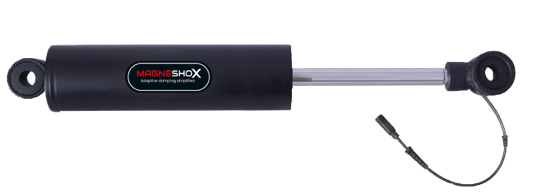
\includegraphics[height=3cm]{Figures/MagnetorheologicalShockAbsorber.png}
            \caption{Arus MR Tech’s “Magneshox” magnetorheological damper \cite{ArusMR_Magneshox}.}
            \label{fig:MagnetorheologicalShockAbsorber} 
        \end{figure}
        \vspace{-20pt} % Adjust this value to reduce the space
        \FloatBarrier

        Friction disk dampers, like the one portrayed in Figure \ref{fig:FrictionShockAbsorber}, work, as the name implies, through the friction between a stack of tightly clamped disks. This early form of damper was considered obsolete after more modern ones were developed \cite{Setright1976_Suspension}.

        \renewcommand{\thefigure}{S14}
        \begin{figure}[ht]
            \centering
            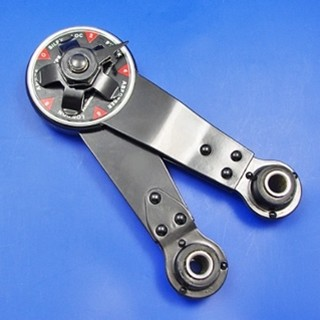
\includegraphics[height=3cm]{Figures/FrictionShockAbsorber.jpg}
            \caption{Andre Hartford friction disk shock absorber - Model 302M \cite{VintageCarParts_AndreHartford}.}
            \label{fig:FrictionShockAbsorber} 
        \end{figure}
        \vspace{-20pt} % Adjust this value to reduce the space
        \FloatBarrier

        Electromagnetic dampers are a type of regenerative shock absorbers; instead of dissipating the energy of the oscillations, they store it as practical energy, such as electricity. This type of system uses an electric generator that consists of a stack of permanent magnets and coils to transform motion into energy \cite{Unitrailer_HydraulicShockAbsorber}. Electromagnets could replace the permanent magnets, allowing for more active control over the damping. Figure \ref{fig:ElectromagneticShockAbsorber} represents a concept for a hydropneumatic shock absorber.

        \renewcommand{\thefigure}{S15}
        \begin{figure}[ht]
            \centering
            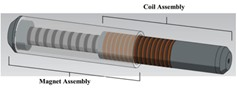
\includegraphics[height=3cm]{Figures/ElectromagneticShockAbsorber.jpg}
            \caption{Concept of an electromagnetic damper \cite{PhysOrg_EnergyRecovery_2010}.}
            \label{fig:ElectromagneticShockAbsorber} 
        \end{figure}
        \vspace{-20pt} % Adjust this value to reduce the space
        \FloatBarrier

        Hydropneumatic shock absorbers combine many of the elements of other suspensions discussed previously to allow for the advantages of both hydraulic and pneumatic suspensions while having the possibility for ride height adjustability. An example of this type of damper is illustrated in Figure \ref{fig:HydroPneumaticShockAbsorber}.

        \renewcommand{\thefigure}{S16}
        \begin{figure}[ht]
            \centering
            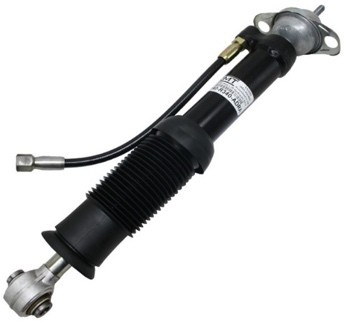
\includegraphics[height=3cm]{Figures/HydroPneumaticShockAbsorber.jpg}
            \caption{Mercedes Benz’s s-class w140 hydropneumatic self-levelling shock absorber \cite{RebuildMasterTech_OE_Rebuilt_ShockAbsorber}.}
            \label{fig:HydroPneumaticShockAbsorber} 
        \end{figure}
        \vspace{-20pt} % Adjust this value to reduce the space
        \FloatBarrier

        Hysteresis dampers rely solely on the tendency for elastic materials to rebound from a deformation with less force than the one that caused it. These materials can be rubber disks, bands, cords, or mechanical springs \cite{RebuildMasterTech_OE_Rebuilt_ShockAbsorber}.

\subsection{Concept Generation Phase I}
    Apart from the main concepts presented in the report (C1, C3, C8, and C10), this section of the repository includes the remaining six concepts illustrated in Figures \ref{fig:C2} to S22.

    \renewcommand{\thefigure}{S17}
    \begin{figure}[ht]
        \centering
        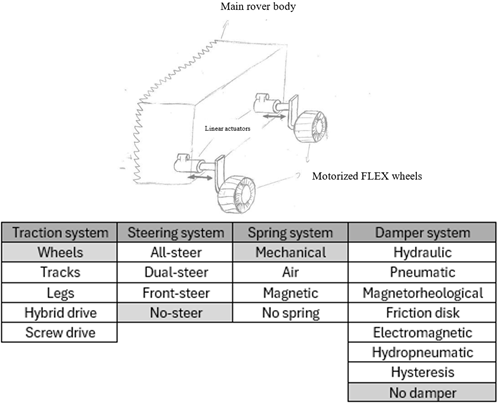
\includegraphics[height=8.5cm]{Figures/C2.png}
        \caption{Second concept generated (C2).}
        \label{fig:C2} 
    \end{figure}
    \vspace{-20pt} % Adjust this value to reduce the space
    \FloatBarrier

    \renewcommand{\thefigure}{S18}
    \begin{figure}[ht]
        \centering
       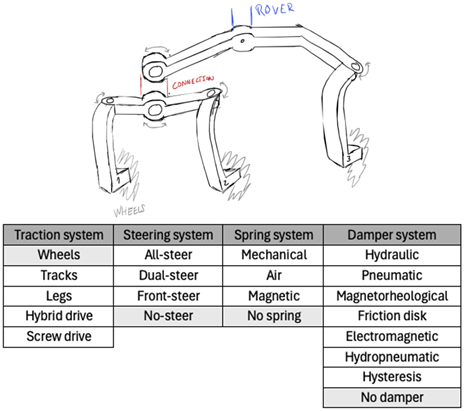
\includegraphics[height=8.5cm]{Figures/C4.png}
       \caption{Fourth concept generated (C4).}
       \label{fig:C4} 
    \end{figure}
    \vspace{-20pt} % Adjust this value to reduce the space
    \FloatBarrier

    \renewcommand{\thefigure}{S19}
    \begin{figure}[ht]
        \centering
        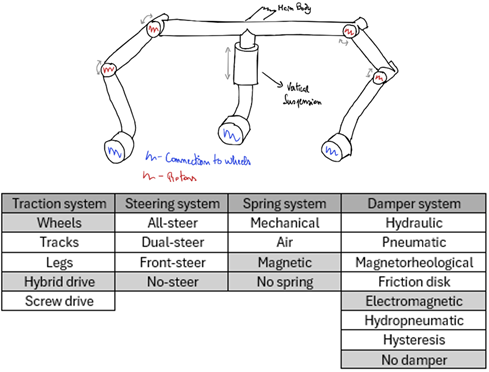
\includegraphics[height=8.5cm]{Figures/C5.png}
       \caption{Fifth concept generated (C5).}
       \label{fig:C5} 
    \end{figure}
    \vspace{-20pt} % Adjust this value to reduce the space
    \FloatBarrier

    \renewcommand{\thefigure}{S20}
    \begin{figure}[ht]
        \centering
        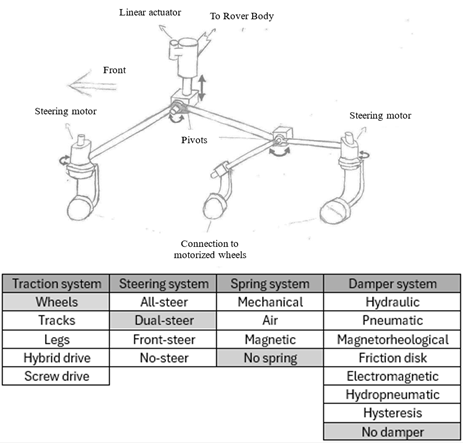
\includegraphics[height=8.5cm]{Figures/C6.png}
        \caption{Sixth concept generated (C6).}
        \label{fig:C6} 
    \end{figure}
    \vspace{-20pt} % Adjust this value to reduce the space
    \FloatBarrier

    \renewcommand{\thefigure}{S21}
    \begin{figure}[ht]
        \centering
        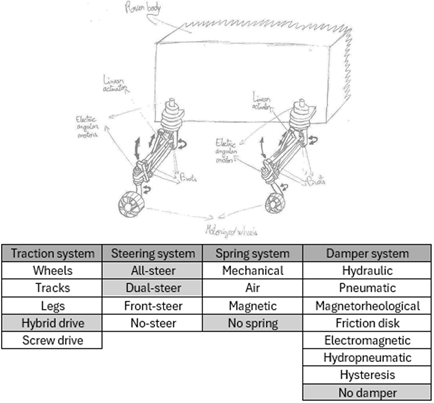
\includegraphics[height=8.5cm]{Figures/C7.png}
        \caption{Seventh concept generated (C7).}
        \label{fig:C7} 
    \end{figure}
    \vspace{-20pt} % Adjust this value to reduce the space
    \FloatBarrier

    \renewcommand{\thefigure}{S22}
    \begin{figure}[ht]
        \centering
        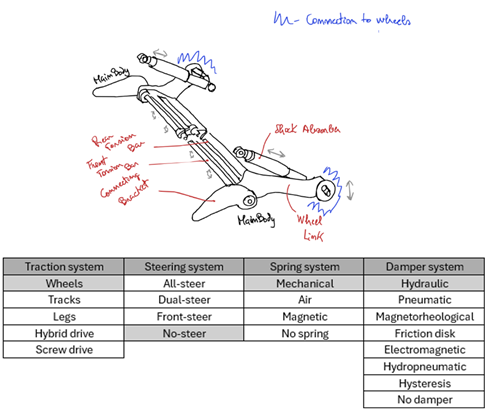
\includegraphics[height=8.5cm]{Figures/C9.png}
        \caption{Ninth concept generated (C9).}
        \label{fig:C9} 
    \end{figure}
    \vspace{-20pt} % Adjust this value to reduce the space
    \FloatBarrier

    \renewcommand{\thesection}{S5}
\section{Material Selection}
\setcounter{subsection}{4}
\subsection{Ranking}
    From the previously defined constraints (presented in Table 6 of the main report), 59 materials from the databases satisfied the set restrictions. All these materials were part of the metals family and included aluminium alloys, titanium alloys, nickel-titanium alloys, nickel-chromium alloys, chromium metal, zirconium alloys, among others. The evaluation focused on yield strength and density to rank the materials effectively.
    
    A performance index, shown in equation \ref{eq:performance}, was derived from equation 1 of the main report to refine the analysis further and applied to generate an Ashby plot for the previously mentioned materials, this plot is represented in Figure 16 of the main report. This plot facilitated visualization and comparison of material performance based on the performance index.

    \renewcommand{\theequation}{S2}
    \begin{equation}
        \log(\sigma) = \frac{3}{2}\left(\log(\rho) + \log(P_{\text{cr}})\right)
        \label{eq:performance}
    \end{equation}

    This equation allowed for the plotting of lines with a constant slope which served as a tool to ascertain the materials with the highest $P_{cr}$ (the highest the value of the line at $x=0$, the highest the $P_{cr}$).

    \renewcommand{\thesection}{S6}
\section{Design of the Rover Suspension System}

\subsection{Force Distribution}
    For this section many calculations were performed, calculations which were not to be present in the main report, as such, Figure \ref{fig:ForceCalculations} presents these calculations in a more step-by-step basis.

    \renewcommand{\thefigure}{S23}
    \begin{figure}[ht]
        \centering
        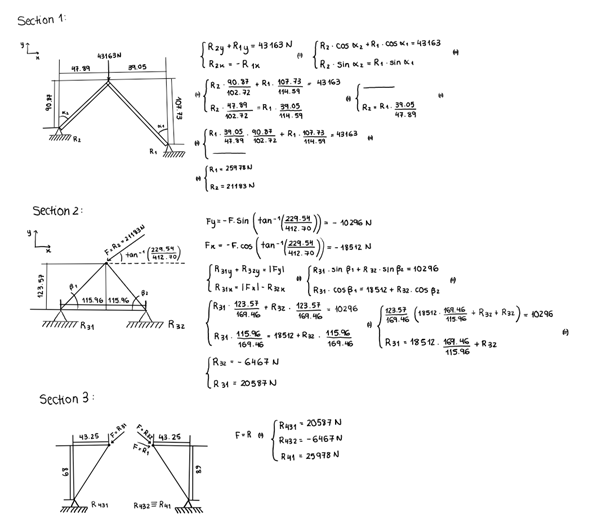
\includegraphics[height=13cm]{Figures/ForceCalculations.png}
        \caption{Calculations performed in the Force Distribution subsection of the main report.}
        \label{fig:ForceCalculations} 
    \end{figure}
    \vspace{-20pt} % Adjust this value to reduce the space
    \FloatBarrier

    \renewcommand{\thesection}{S7}
\section{Simulation Results and Validation}

\subsection{Static Simulations}
    For both static simulations in which the structure was subjected to launch-phase conditions with 8g of acceleration, a mesh convergence study was conducted. Figure \ref{fig:MeshConvergence} presents a graph of the maximum von Mises stress (MPa) versus the number of mesh elements, showing that the results stabilize with mesh refinement. This confirms the validity of the obtained stress values. The blue curve corresponds to the I-beam profile, and the orange curve to the manufacturable version.

    \renewcommand{\thefigure}{S24}
    \begin{figure}[ht]
        \centering
        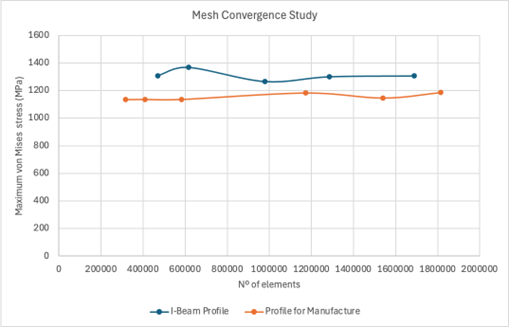
\includegraphics[height=6cm]{Figures/MeshConvergence.png}
        \caption{Maximum von Mises stress vs. number of elements for static simulations under launch-phase loading (8g), showing convergence for the I-beam (blue) and manufacturable profile (orange).}
        \label{fig:MeshConvergence} 
    \end{figure}
    \vspace{-20pt} % Adjust this value to reduce the space
    \FloatBarrier

    For the same simulation, Figure \ref{fig:Displacement} shows the maximum displacement (URES, total resultant displacement, in millimetres), with the I-beam on the left and the manufacturable configuration on the right. The results indicate peak values of 17 mm and 32 mm, respectively. It is also worth noting that the maximum displacement values consistently converged with mesh refinement, as previously discussed.

    \renewcommand{\thefigure}{S25}
    \begin{figure}[ht]
        \centering
        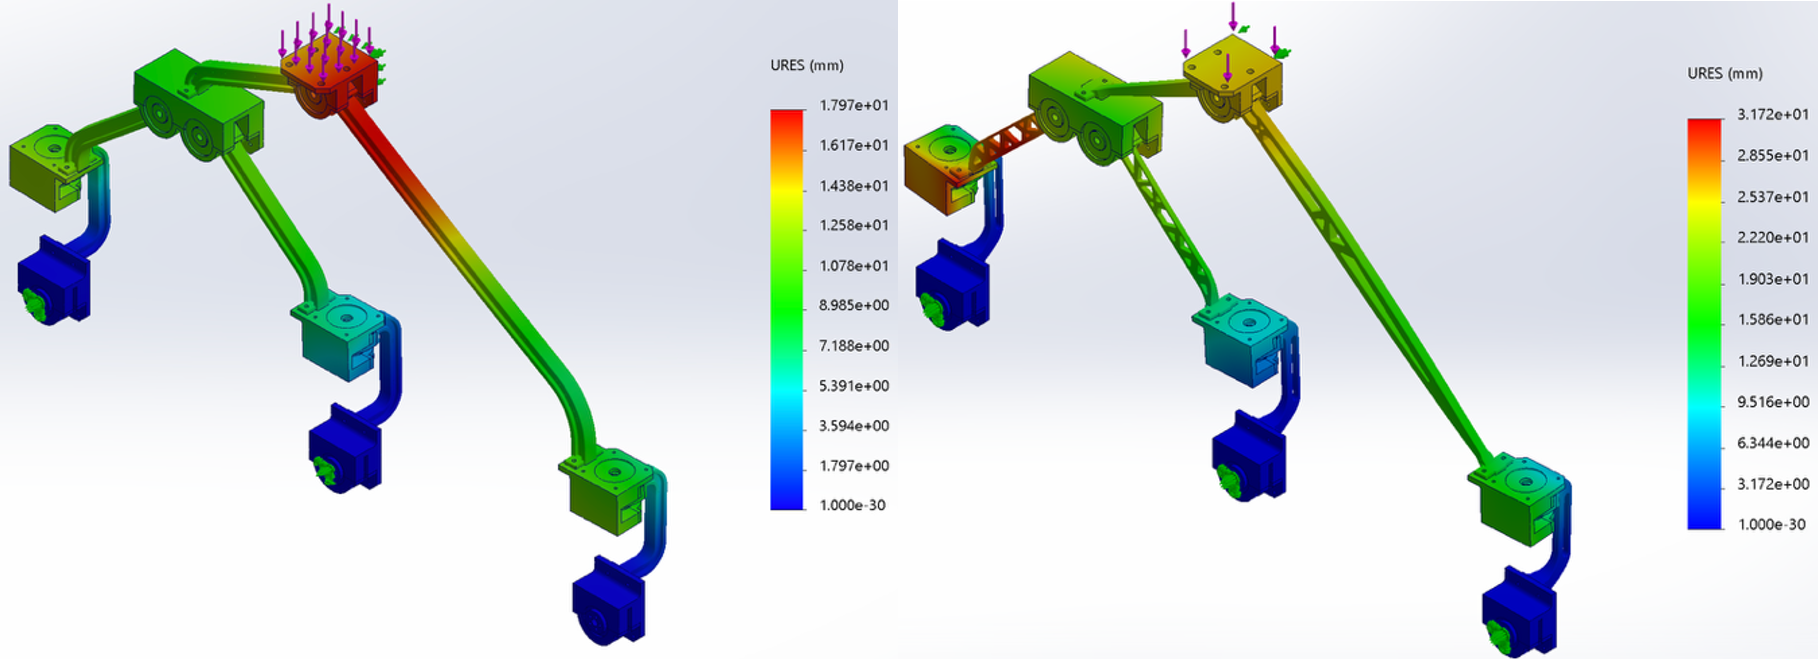
\includegraphics[height=5.5cm]{Figures/Displacement.png}
        \caption{Maximum displacement (URES) from static simulations under launch-phase loading (8g). Comparison between the I-beam (left) and manufacturable configuration (right).}
        \label{fig:Displacement} 
    \end{figure}
    \vspace{-20pt} % Adjust this value to reduce the space
    \FloatBarrier

    \clearpage % Start bibliography on a new page
    \renewcommand{\bibname}{Bibliography} % Ensure the title matches the section formatting
    \addcontentsline{toc}{section}{Bibliography} % Add to Table of Contents
    \bibliography{Bibliography} % Link to your .bib file

\end{document}
